\documentclass{exam}
\usepackage{../../commonheader}

%%% CHANGE THESE %%%%%%%%%%%%%%%%%%%%%%%%%%%%%%%%%%%%%%%%%%%%%%%%%%%%%%%%%%%%%%
\discnumber{4}
\title{\textsc{Nonlocality and Object-Oriented Programming}}
\date{February 29 to March 5, 2016}
%%%%%%%%%%%%%%%%%%%%%%%%%%%%%%%%%%%%%%%%%%%%%%%%%%%%%%%%%%%%%%%%%%%%%%%%%%%%%%%

\begin{document}
\maketitle
\rule{\textwidth}{0.15em}
\fontsize{12}{15}\selectfont

%%% INCLUDE TOPICS HERE %%%%%%%%%%%%%%%%%%%%%%%%%%%%%%%%%%%%%%%%%%%%%%%%%%%%%%%


%%% Question %%%

\begin{questions}
\begin{blocksection}
\question \textbf{(H)OOP} \newline
Given the following code, what will Python output for the following prompts? 

\begin{lstlisting}
class Baller:
    all_players = []
    def __init__(self, name, has_ball = False):
       self.name = name
       self.has_ball = has_ball
       Baller.all_players.append(self)
    
    def pass_ball(self, other_player):
       if self.has_ball:
          self.has_ball = False
          other_player.has_ball = True
          return True
       else:
          return False

class BallHog(Baller):
    def pass_ball(self, other_player):  
       return False 
       
\end{lstlisting}

\begin{lstlisting}
>>> tiffany = Baller('Tiffany', True)
>>> jerry = BallHog('Jerry')
>>> len(Baller.all_players)
\end{lstlisting}
\begin{solution}[.2in]
2
\end{solution}

\begin{lstlisting}
>>> Baller.name
\end{lstlisting}
\begin{solution}[.2in]
Error
\end{solution}

\begin{lstlisting}
>>> len(jerry.all_players)
\end{lstlisting}
\begin{solution}[.2in]
2
\end{solution}
\end{blocksection}

\begin{blocksection}
\begin{lstlisting}
>>> tiffany.pass_ball()
\end{lstlisting}
\begin{solution}[.2in]
Error
\end{solution}

\begin{lstlisting}
>>> tiffany.pass_ball(jerry)
\end{lstlisting}
\begin{solution}[.2in]
True
\end{solution}

\begin{lstlisting}
>>> tiffany.pass_ball(jerry)
\end{lstlisting}
\begin{solution}[.2in]
False
\end{solution}

\begin{lstlisting}
>>> BallHog.pass_ball(jerry, tiffany)
\end{lstlisting}
\begin{solution}[.2in]
False
\end{solution}

\begin{lstlisting}
>>> jerry.pass_ball(tiffany)
\end{lstlisting}
\begin{solution}[.2in]
False
\end{solution}

\begin{lstlisting}
>>> jerry.pass_ball(jerry, tiffany)
\end{lstlisting}
\begin{solution}[.2in]
Error
\end{solution}
\end{blocksection}

%%% Question %%%
\begin{blocksection}
\question \textbf{TeamBaller} \newline
Write \texttt{TeamBaller}, a subclass of \texttt{Baller}. An instance of \texttt{TeamBaller} cheers on the team every time it passes a ball.  \newline
Hint: What can we use to avoid writing duplicate code? \newline
"Super" Hint: There are two ways to implement \texttt{pass\_ball} \newline

\begin{lstlisting}
>>> cheerballer = TeamBaller('Susanna', has_ball=True)
>>> cheerballer.pass_ball(jerry)
Yay!!!!
True
>>> cheerballer.pass_ball(jerry)
I dont have the ball :(
False


class TeamBaller(_________):
    def pass_ball(_________, __________):
        """*** Enter solution below ***"""
\end{lstlisting}
\begin{solution}[1in]
\begin{lstlisting}
class TeamBaller(Baller):
    def pass_ball(self, other_player):
        did_pass = super().pass_ball(other_player) 
        # above line could also be:
        # did_pass = Baller.pass_ball(self, other_player)
        if did_pass:
            print('Yay!!!!')
        else:
            print("I dont have the ball :(")
\end{lstlisting}
\end{solution}
\end{blocksection}

%%% Question %%%

\begin{blocksection}
\question \textbf{Nonlocal Kale} \newline
Draw the environment diagram for the following code.

\begin{lstlisting}
eggplant = 8
carrot = 0
def vegetable(kale):
    carrot = 10
    def eggplant(spinach):
        nonlocal eggplant
        nonlocal kale
        kale = 9
        carrot = 20
        eggplant = spinach
    eggplant(kale)
    return eggplant
spinach = vegetable(lambda kale: carrot*kale)(eggplant)
\end{lstlisting}

\begin{solution}[3in]
    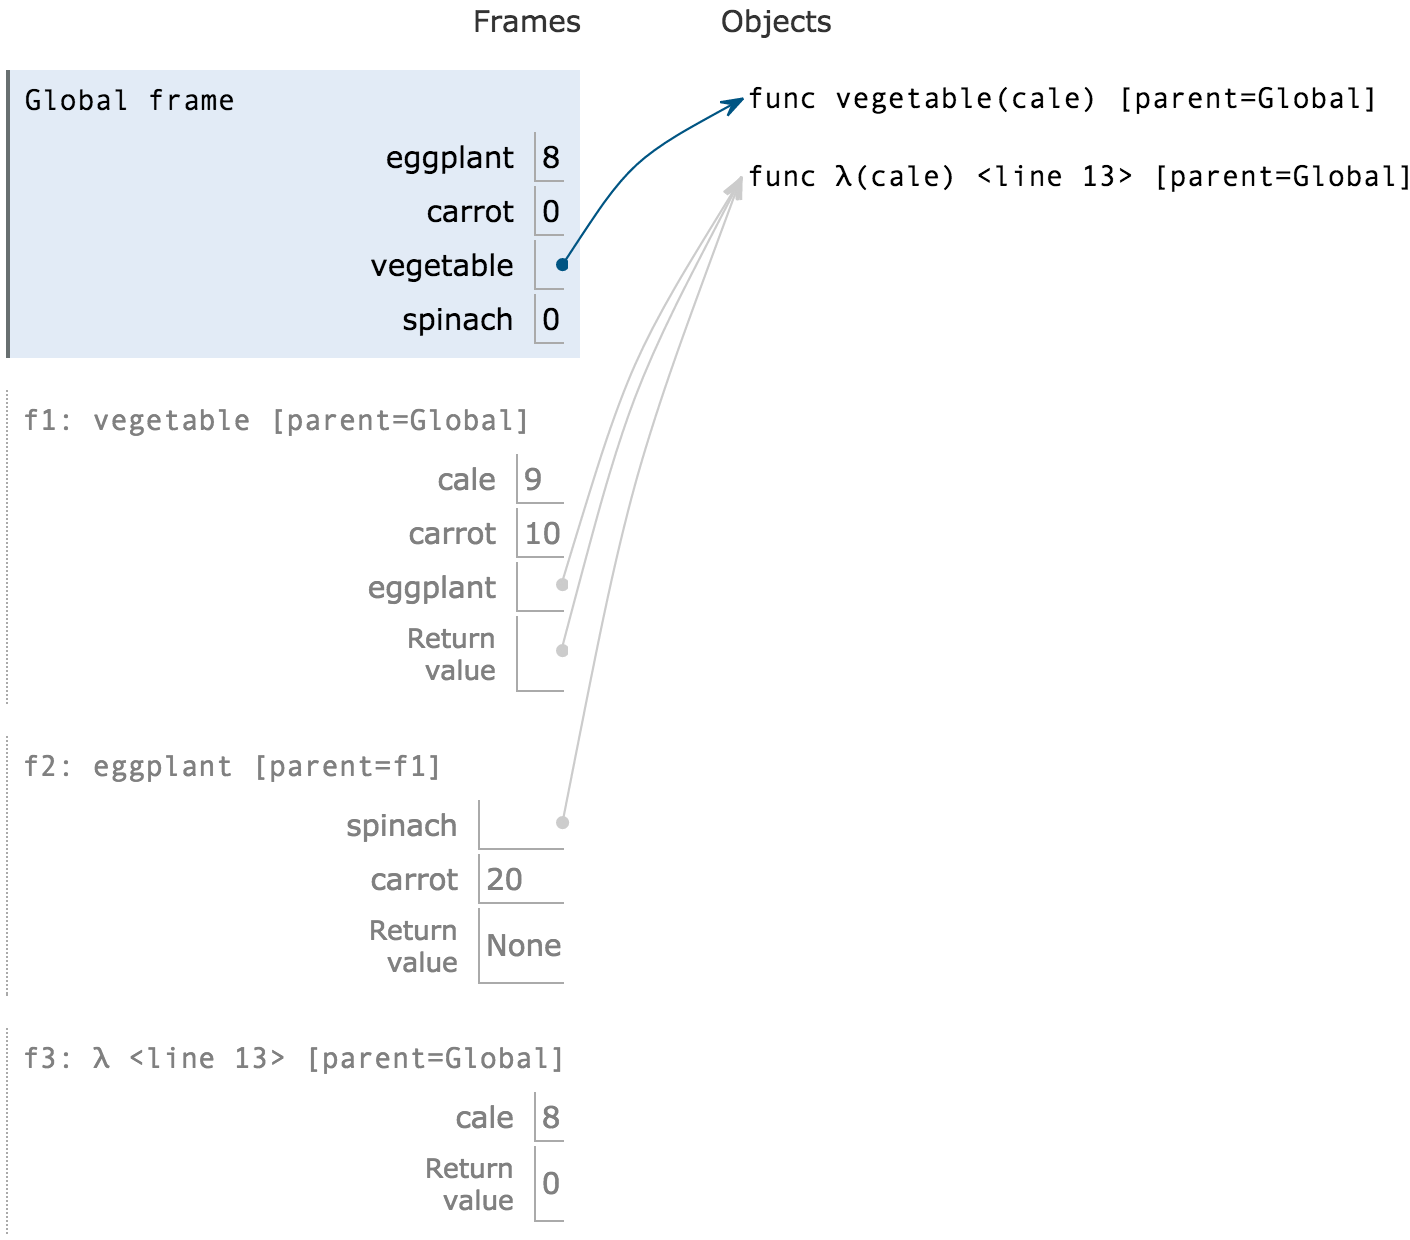
\includegraphics[scale=0.5]{img/kale.png}
\end{solution}

\end{blocksection}

\begin{blocksection}
\question \textbf{Pinpong again...}  \newline
Recap of ping-pong: The ping-pong sequence counts up starting from 1 and is always either counting up or counting down. At element k, the direction switches if k is a multiple of 7 or contains the digit 7. The first 30 elements of the ping-pong sequence are listed below, with direction swaps marked using brackets at the 7th, 14th, 17th, 21st, 27th, and 28th elements:
\begin{lstlisting}
1 2 3 4 5 6 [7] 6 5 4 3 2 1 [0] 1 2 [3] 2 1 0 [-1] 0 1 2 3 4 [5] [4] 5 6
\end{lstlisting}
Implement a function \texttt{make\_pingpong\_tracker} that returns the next value in the pingpong sequence each time it is called.  In the body of \texttt{make\_pingpong\_tracker}, you can use assignment statements.
\newline

\begin{lstlisting}
def has_seven(k): #Use this function for your answer below
    if k % 10 == 7:
        return True
    elif k < 10:
        return False
    else:
        return has_seven(k // 10)

def make_pingpong_tracker():
    """ Returns a function that returns the next value in the pingpong sequence
    each time it is called.
    >>> output = []
    >>> x = make_pingpong_tracker()
    >>> for _ in range(9):
    ... output += [x()]
    >>> output
    [1, 2, 3, 4, 5, 6, 7, 6, 5]
    """
    index, current, add = 1, 0, True
    def pingpong_tracker():
        __________________________
        if add:
            ________________________
        else:
            ________________________
        if _______________________:
            add = not add
        __________________________
        __________________________
    return pingpong_tracker

\end{lstlisting}

\begin{solution}
\begin{lstlisting}
def make_pingpong_tracker():
    index, current, add = 1, 0, True
    def pingpong_tracker():
        nonlocal index, current, add
        if add:
            current = current + 1
        else:
            current = current - 1
        if has_seven(index) or index % 7 == 0:
            add = not add
        index += 1
        return current
    return pingpong_tracker
\end{lstlisting}
\end{solution}

\end{blocksection}

\begin{blocksection}
\question \textbf{(Optional)} Instead of using nonlocal for pingpong, let's use OOP!

\begin{lstlisting}
>>> tracker1 = PingPongTracker()
>>> tracker2 = PingPongTracker()
>>> tracker1.next()
1
>>> tracker1.next()
2
>>> tracker2.next()
1

Bonus points if you can get the following syntax.
>>> tracker1()
1
>>> tracker1()
2

class PingPongTracker:
    def __init__(self):
        self.current = 0
        self.index = 1
        self.add = True
    def next(self):
        """*** Enter solution below ***"""
\end{lstlisting}

\begin{solution}[0.3in]
\begin{lstlisting}
class PingPongTracker:
    def __init__(self):
        self.current = 0
        self.index = 1
        self.add = True

    def next(self):
        if self.add:
            self.current += 1
        else:
            self.current -= 1
        if has_seven(self.index) or self.index % 7 == 0:
            self.add = not self.add
        self.index += 1
        return self.current


Notice how the OOP approach is insanely similar to the non local function. Instead of using nonlocal, we use self.varName and the code becomes exactly the same. We just store the data in a slightly different way. This implies that OOP and functions are pretty similar, and it turns out you can even write your own OOP framework using just functions and nonlocal! 
In addition, there are a lot of python specific features that can be written using functions or using classes. If you are interested, check out the powerful python feature decorators, and note how we can write them both as functions and as classes!
\end{lstlisting}
\end{solution}

\end{blocksection}

\end{questions}

%%%%%%%%%%%%%%%%%%%%%%%%%%%%%%%%%%%%%%%%%%%%%%%%%%%%%%%%%%%%%%%%%%%%%%%%%%%%%%%

\end{document}
